\documentclass[reprint,english,notitlepage]{revtex4-1}
% if you want a single-column, remove reprint

% allows special characters (including æøå)
\usepackage[utf8]{inputenc}
%\usepackage [norsk]{babel} %if you write norwegian
\usepackage[english]{babel}  %if you write english


\usepackage{physics,amssymb}  % mathematical symbols (physics imports amsmath)
\usepackage{graphicx}         % include graphics such as plots
\usepackage{xcolor}           % set colors
\usepackage{hyperref}         % automagic cross-referencing (this is GODLIKE)
\usepackage{tikz}             % draw figures manually
\usepackage{listings}         % display code
\usepackage{subfigure}        % imports a lot of cool and useful figure commands
\usepackage{float}			  % force placement of tables and figures
\usepackage{amsmath}
\usepackage{minted}

\hypersetup{ % this is just my personal choice, feel free to change things
	colorlinks,
	linkcolor={red!50!black},
	citecolor={blue!50!black},
	urlcolor={blue!80!black}}

%% Defines the style of the programming listing
%% This is actually my personal template, go ahead and change stuff if you want
\lstset{ %
	inputpath=,
	backgroundcolor=\color{white!88!black},
	basicstyle={\ttfamily\scriptsize},
	commentstyle=\color{magenta},
	language=Python,
	morekeywords={True,False},
	tabsize=4,
	stringstyle=\color{green!55!black},
	frame=single,
	keywordstyle=\color{blue},
	showstringspaces=false,
	columns=fullflexible,
	keepspaces=true}

\begin{document}
	
\title{Studying the Ising model using the Metropolis algorithm \\
	\normalsize FYS4150 - Prosjekt 4}
\date{\today}               
\author{Karl Henrik Fredly}
\affiliation{Universitetet i Oslo} 

\newpage
	
\begin{abstract} %------------------Abstract-----------------------
	In this project we are going to study the Ising model using the Metropolis algorithm.
	
	We will first look at how the algorithm performs on the 2x2 Ising model compared to analytical solutions, and how parallellization can speed up the algorithm by around 4.4 times. Then, we will see how its results for a 20x20 model compares with our expectations, and specifically how the results for a low temperature differ from those for a high temperature.
	
	Finally, we will study the phase transition that happens around the critical temperature of the system, and predict the critical temperature of an Ising model with an infinite lattice. By looking at the spike in heat capacity around the critical temperature of models of different sizes, we predict a critical temperature of an infinite lattice of $T_C(L = \infty) = 2.2699 J/k_B$, a value only $0.0007J/k_B$ away from the analytical result of $T_C(L = \infty) \approx 2.2692 J/k_B$. Our result has some uncertainty to it however, as is shown by our prediction using the same method only with spikes in magnetic susceptibility having an error of $0.0023J/k_B$.
	
	- Github repository with code and results:
	
	 \href{https://github.com/KarlHenrik/ComputationalPhysicsMaster/tree/master/FYS4150/Project5}{https://github.com/KarlHenrik/ComputationalPhysicsMaster/tree/master/FYS4150/Project5}
\end{abstract}
\maketitle

\section{Introduction} %------------------Introduksjon-----------------------
	The Ising model is a physical model which allows us to model phase transitions in materials consisting of many degrees of freedom, like atoms in a lattice structure, each with their own magnetic moment. We will look at the two dimentional Ising model in this project, which was solved analytically by the norwegian Lars Onsager in 1944. Even though it has been solved analytically, it is an interesting problem to look at numerically, as it lends itself well to being analyzed with the Monte Carlo method the Metropolis algorithm.

	In the methods section, we give a short introduction to the Ising model, presenting the central formulas and physical properties of the model, and the properties we will try to approximate in our calculation. We present the central properties of the Metropolis algorithm, and the practicalities of how it will be used in our specific use case. We then present analytical results for a 2x2 Ising model we can use to test our code.
	
	Then, in the results section we present the results of our calculations, and the parameters that produced them.
	
	Finally, in the discussion and conclusion, we relate our results to the theory we discussed in the methods section, what they show us about the Ising model, and how the Metropolis algorithm performed in reproducting analytical results.
	
	All code used for this project was written by me \cite{myRepo}, including structuring of the Ising model and implementation of the Metropolis algorithm.

\section{Methods} %------------------Metoder-----------------------
	
\subsection{The Ising model}
	The Ising model aims to model the properties of a structure consisting of a large number of magnetic dipole moments of atomic spins. In this project, we will use the two dimensional Ising model, where the spins are arranged in a $L\times L$ lattice. The spins can be in the state $+1$ or $-1$, and the spins interact only with their closest neighbors. An example of a possible microstate of a $4 \times 4$ lattice is shown here, with $\uparrow = +1, \downarrow = -1$:
	
	\begin{equation*}
	\begin{aligned}
	\downarrow \uparrow \uparrow \downarrow \\
	\uparrow \uparrow \uparrow \downarrow \\
	\downarrow \uparrow \downarrow \uparrow \\
	\downarrow \downarrow \uparrow \uparrow
	\end{aligned}
	\end{equation*}
	
	Since each spin can be in two states, the lattice can be in $2^N$ different microstates, where $N$ is the number of spins. The problem then, when we are studying the properties of a lattice with a non-trivial number of spins, is that there are too many possible microstates to analyze them all. The solution is to start in a random state, and to then perform a random walk following the Metropolis algorithm, which lets us extract many useful statistical properties of the system.
	
	Before we look at the Metropolis algorithm however, we must look at some useful properties of the Ising model, and which properties of interest we will be approximating. For a more thorough explanation, see \cite{compfys}.

	The energy of a particular microstate is given by
	\begin{equation}
	\label{eq:E}
	\begin{aligned}
	&E = -J \sum_{<k,l>}^{N} s_k s_l
	\end{aligned}
	\end{equation}
	where $N$ is the number of spins, $J (> 0)$ describes the strength of the interaction between spins, $s_k$ and $s_l$ are two spins in the lattice, and $<k,l>$ signifies that we only sum over nearest neighbors. At the edge of the lattice, each spin is assumed to be connected to the spin at the opposite end of the lattice, this is called periodic boundary conditions.
	
	The probability of being in a particular microstate $i$ is given by
	\begin{equation}
	\label{eq:P}
	\begin{aligned}
	&P_i = \frac{1}{Z} e^{-E_i \beta}
	\end{aligned}
	\end{equation}
	where $E_i$ is the energy of the microstate, and $\beta = 1/k_BT$, where $k_B$ is Boltzmann's constant and $T$ is the temperature. $Z$ is the partition function of the system, given by
	\begin{equation}
	\label{eq:Z}
	\begin{aligned}
	&Z = \sum_{i}^G e^{-\beta E_i}
	\end{aligned}
	\end{equation}
	where $G$ is the number of possible mictostates. Z helps normalize the probability, but is impractical to calculate for systems with a non-trivial number of spins. Note that the ratio of probabilities of two microstates does not require Z to calculate
	\begin{equation}
	\label{eq:Pt}
	\begin{aligned}
	\frac{P_i}{P_j} = \frac{e^{-E_i \beta}/Z}{e^{-E_j \beta}/Z} = e^{(Ej - E_i) \beta}
	\end{aligned}
	\end{equation}
	This will be useful in the Metropolis algorithm. The magnetization of a microstate is given by
	\begin{equation}
	\begin{aligned}
	\label{eq:M}
	&M = \sum_{i}^N s_i
	\end{aligned}
	\end{equation}
	We will approximate the following properties in our calculations
	\begin{equation}
	\label{eq:evs}
	\begin{aligned}
		\expval{E} &= \frac{1}{Z} \sum_{i}^{G} E_i e^{-E_i \beta} \\
		\expval{E^2} &= \frac{1}{Z} \sum_{i}^{G} E_i^2 e^{-E_i \beta} \\
		\expval{|M|} &= \frac{1}{Z} \sum_{i}^{G} |M|_i e^{-E_i \beta} \\
		\expval{M^2} &= \frac{1}{Z} \sum_{i}^{G} M_i^2 e^{-E_i \beta} \\
		C_V &= \frac{1}{k_B T^2} (\expval{E^2} - \expval{E}^2) \\
		\chi &= \frac{1}{k_B T} (\expval{M^2} - \expval{|M|}^2)
	\end{aligned}
	\end{equation}
	The final property of interest is the critical temperature $T_C$. It is the temperature where the properties of the system undergo rapid change, where the system undergoes a phase transition. Below the critical temperature, the Ising model is spontaneously magnetized, due to the spins mostly aligning in the same direction. Above the critical temperature, the magnetization disappears, as the spins are no longer nearly as aligned.
	
	The critical temperature for a given lattice size $L$ ($L$ is the number of spins in each direction of the $L \times L$ lattice) is characterized by a rapid drop in magnetization, a spike in heat capacity $C_V$ and magnetic susceptibility $\chi$, and a rapid increase in energy. We will use the spikes in heat capacity and magnetic susceptibility to find the critical temperature for different lattice sizes.
	
	The critical temperature for an infinite lattice is connected to the critical temperature for a lattice of size $L$ through the relation
	\begin{equation}
	\label{eq:tc}
	\begin{aligned}
	&T_C(L) = T_C(L=\infty) + \frac{a}{L}
	\end{aligned}
	\end{equation}
	We will attempt to approximate $T_C(L=\infty)$, which has an analytical value of $\approx2.269$ by doing a linear fit to our values of $T_C(L)$.
	
	The increased misalignment of spins for higher temperatures can be explained by the increased entropy $S$ of the system. An important property for this system is the Helmholtz Free Energy $F$:
	\begin{equation}
	\label{eq:helmholtz}
	\begin{aligned}
	F = \expval{E} - TS
	\end{aligned}
	\end{equation}
	$F$ will always "try" to be minimized for this system. This dynamic describes the trade-off between minimizing the energy of the system and maximizing the entropy.
	
\subsection{The Metropolis algorithm}
	We will present a gross simplification of the Metropolis algorithm, which only aims to capture the practicalities of the algorithm relevant to our calculations. For a more thorough explanation, see \cite{compfys}.
	
	The Metropolis algorithm lets us perform a random walk between possible microstates of the system, which after a large number of steps results in the visited microstates being representative of all the possible microstates. This means that the statistical properties discussed in the previous section can be approximated by performing a random walk with the Metropolis algorithm.
	
	In order for the visited states to be statistically representative, we need the probability of the system changing from a state $j$ to a neighboring state $i$. A neighboring state is a state where only a single spin is flipped, compared to the original state. We only look at transitions to neighboring states, as we then only have 5 possible energy transitions. The spin $s_0$ with neighbors $s_1, s_2, s_3$ and $s_4$ contributes the energy $e = -J s_0(s_1 + s_2 + s_3 + s_4)$. If we now flip $s_0$, the energy contribution becomes $-e$, as $s_0$ changed its sign. $e$ can only take the values $4J, 2J, 0J, -2J, -4J$, so $\Delta E = -2e$ can only take the values $8J, 4J, 0J, -4J, -8J$.
	
	We model the probability of transitioning from a state $j$ to a neighboring state $i$ $P(j \rightarrow i)$ as $1$ if the energy change is negative, as we are moving to a more likely state (from equation \ref{eq:P}). If the state $i$ we are transitioning to has a higher energy however, we use the ratio of the probabilities of being in the two states from equation \ref{eq:Pt}
	\begin{equation*}
	\begin{aligned}
	P(j \rightarrow i) = \frac{P_i}{P_j} = \frac{e^{-E_i \beta}/Z}{e^{-E_j \beta}/Z} = e^{(Ej - E_i) \beta} = e^{\Delta E \beta}
	\end{aligned}
	\end{equation*}
	Since $\Delta E$ can only take 5 different values for a given temperature, we can precompute the transition probabilities $P(j \rightarrow i)$ before simulating the random walk to make the algorithm much more efficient.
	
	The Metropolis algorithm then works as follows:
	
	$\bullet$ Initialize the lattice in a random state and calculate the energy and magnetic moment, together with the possible $\Delta E$ values
	
	$\bullet$ Suggest a random transition $j \rightarrow i$ to a neighboring state, and accept the transition with probability $P(j \rightarrow i)$. If you transitioned, compute the new energy and magnetic moment. Update expectation values after each sweep through the lattice ($L^2$ suggestions), and repeat for a given number of cycles.
	
	The algorithm is very slow, as it takes a large number of cycles to reach a representative selection of microstates, so we parallelized it to save time. We chose to let each thread perform the metropolis algorithm for a different temperature.
	
	When performing the Metropolis algorithm and calculating the various expected values, we are interested in visiting a mix of microstates that follow the probability distribution of the system. The random initial state skews the expected values, as it was "chosen" by us, and not the probability distribution. Therefore, we should discard the first cycles of the program, to ensure our results are not skewed by the initial state. We end up discarding the first 10000 cycles in all of our calculations.
	
\subsection{The 2x2 lattice}
	A 2x2 lattice has few enough spins that we can simply go through the microstates and find their probabilities, energies and magnetic moments by hand. The different microstates are summarized in table \ref{tab:2x2}.
	\begin{table}[H]
		\begin{center}
			\caption{The different microstates of a 2x2 lattice.}
			\label{tab:2x2}
			\begin{tabular}{|c|c|c|c|} \hline
				\textbf{Spin up} & \textbf{Degeneracy} & \textbf{E} & \textbf{M} \\ \hline
				4 & 1 & -8 & 4 \\
				3 & 4 & 0 & 2 \\
				2 & 4 & 0 & 0 \\
				2 & 2 & 8 & 0 \\
				1 & 4 & 0 & -2 \\
				0 & 1 & -8 & -4 \\ \hline
			\end{tabular}
		\end{center}
	\end{table}
	We then find analytical expressions for the different expected values by writing out equations \ref{eq:Z} and \ref{eq:evs}.
	\begin{equation}
	\label{eq:2x2}
	\begin{aligned}
		Z &= 2e^{-8\beta} + 2e^{8\beta} + 12 \\
		\expval{E} &= \frac{1}{Z} (8 * 2e^{-8\beta} - 8 * 2e^{8\beta}) \\
		\expval{E^2} &= \frac{1}{Z} (64 * 2e^{-8\beta} + 64 * 2e^{8\beta}) \\
		\expval{|M|} &= \frac{1}{Z} (4 * 2e^{8\beta} + 2 * 8) \\
		\expval{M^2} &= \frac{1}{Z} (16 * 2e^{8\beta} + 4 * 8) \\
		C_V &= \frac{1}{k_B T^2} (\expval{E^2} - \expval{E}^2) \\
		\chi &= \frac{1}{k_B T} (\expval{M^2} - \expval{|M|}^2)
	\end{aligned}
	\end{equation}
	We will use these results to test our code.
	
\section{Results} %------------------Resultater-----------------------
	
\subsection{Testing and benchmarks}
	We ran our simulations for a 2x2 lattice with 100000 cycles (we discarded the first 10000). The results are shown together with the analytical results from equations \ref{eq:2x2} in figures \ref{fig:2x2E}, \ref{fig:2x2M}, \ref{fig:2x2Cv} and \ref{fig:2x2X}.
	\begin{figure}[H]
		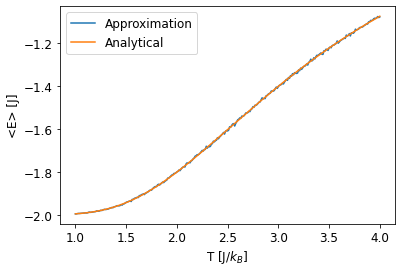
\includegraphics[width=80mm]{../../Code/Figures/2x2E.png}
		\caption{Expected value for the energy per spin of the 2x2 ising model found analytically and with the metropolis algorithm with 100000 cycles.}
		\label{fig:2x2E}
	\end{figure}

	\begin{figure}[H]
		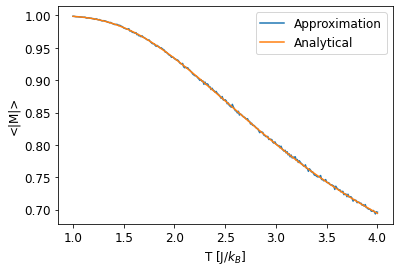
\includegraphics[width=80mm]{../../Code/Figures/2x2M.png}
		\caption{Expected value for the absolute value of the magnetization per spin of the 2x2 ising model found analytically and with the metropolis algorithm with 100000 cycles.}
		\label{fig:2x2M}
	\end{figure}

	\begin{figure}[H]
		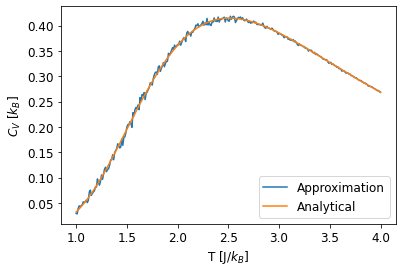
\includegraphics[width=80mm]{../../Code/Figures/2x2Cv.png}
		\caption{Expected value for heat capacity per spin of the 2x2 ising model found analytically and with the metropolis algorithm with 100000 cycles.}
		\label{fig:2x2Cv}
	\end{figure}

	\begin{figure}[H]
		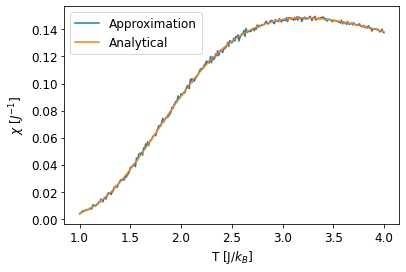
\includegraphics[width=80mm]{../../Code/Figures/2x2X.png}
		\caption{Expected value for the magnetic susceptibility per spin of the 2x2 ising model found analytically and with the metropolis algorithm with 100000 cycles.}
		\label{fig:2x2X}
	\end{figure}

	We then timed our program with and without parallellization. We used 12 parallelized threads.

	\begin{figure}[H]
		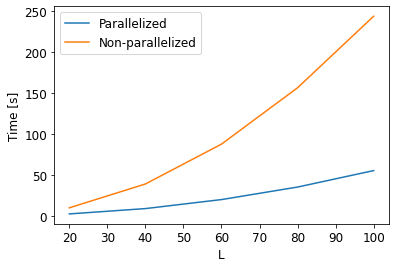
\includegraphics[width=80mm]{../../Code/Figures/time.png}
		\caption{The time it took to perform the Metropolis algorithm with 100000 cycles for different lattice sizes with and without parallelization. We used 12 threads for the parallelization.}
		\label{fig:time}
	\end{figure}

	We found that the parallelized code ran 4.41 $\pm$ 0.05 times faster, that is, a speedup of about 4.4 times.

\subsection{Time to equilibrium}
	To find out how many cycles are needed in order to go from the initial state to the most likely state of the system, we ran the Metropolis algorithm on a $20 \times 20$ lattice and plotted the energy per spin at each cycle in figure \ref{fig:EMC}. We stared in both a state with all spins having random values, and with all spins starting with the value 1.
	\begin{figure}[H]
		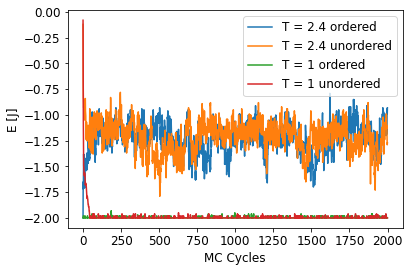
\includegraphics[width=80mm]{../../Code/Figures/EMC.png}
		\caption{The energy per spin of a 20x20 lattice for the first 2000 cycles of the Metropolis algorithm.}
		\label{fig:EMC}
	\end{figure}
	The magnetization per spin at each cycle is shown in figure \ref{fig:MMC}.
	\begin{figure}[H]
		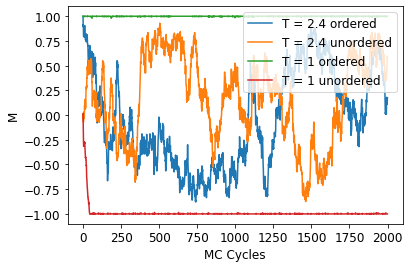
\includegraphics[width=80mm]{../../Code/Figures/MMC.png}
		\caption{The magnetization per spin of a 20x20 lattice for the first 2000 cycles of the Metropolis algorithm.}
		\label{fig:MMC}
	\end{figure}
	The total number of accepted flips at each cycle is shown in figure \ref{fig:AMC}.
	\begin{figure}[H]
		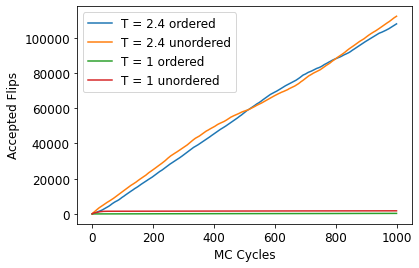
\includegraphics[width=80mm]{../../Code/Figures/AMC.png}
		\caption{The total number of accepted flips for the first 1000 cycles of the Metropolis algorithm for a 20x20 lattice.}
		\label{fig:AMC}
	\end{figure}
	The number of occurences of each energy for cycles 10000-100000 is shown in figure \ref{fig:PE}. The standard deviation of the energy for $T=2.4$ was 0.14J, and for $T=1.0$ it was 0.007J.
	\begin{figure}[H]
		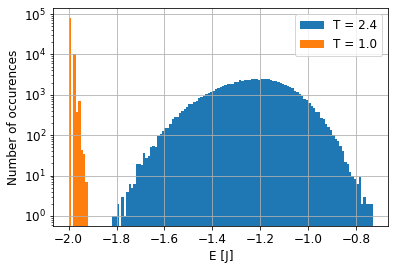
\includegraphics[width=80mm]{../../Code/Figures/PE.png}
		\caption{The number of occurences of each energy per spin for cycles 10000-100000 }
		\label{fig:PE}
	\end{figure}

\subsection{The critical temperature}
	We now take a closer look at how temperature changes the behavior of the system. We ran calculations for T going from from 2.2 to 2.4 in steps of 0.001. Each calculation ran for 1000000 cycles (the first 10000 were discarded like for the 2x2 case. The entire calculation took 7 hours.).
	
	The expected value of temperature per spin for each temperature is shown in figure \ref{fig:E}. 
	\begin{figure}[H]
		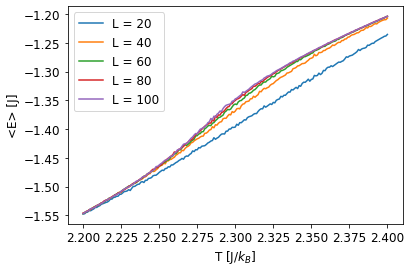
\includegraphics[width=80mm]{../../Code/Figures/E.png}
		\caption{The expected value of energy per spin of a $L \times L$ lattice. The values were calculated with 1000000 sweeps of the lattice with the Metropolis algorithm.}
		\label{fig:E}
	\end{figure}
	The expected value of magnetic moment per spin for each temperature is shown in figure \ref{fig:E}. 
	\begin{figure}[H]
		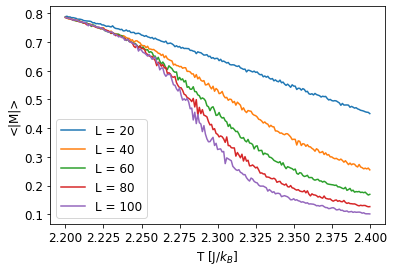
\includegraphics[width=80mm]{../../Code/Figures/M.png}
		\caption{The expected value of the absolute value of the magnetic moment per spin of a $L \times L$ lattice. The values were calculated with 1000000 sweeps of the lattice with the Metropolis algorithm.}
		\label{fig:M}
	\end{figure}
	The acceptance rate of flips per temperature is shown in figure \ref{fig:A}.
	\begin{figure}[H]
		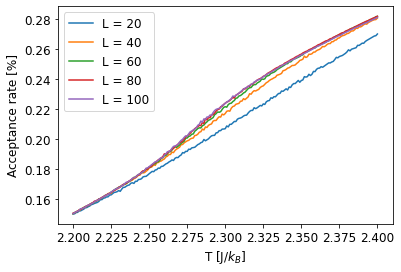
\includegraphics[width=80mm]{../../Code/Figures/A.png}
		\caption{The acceptance rate of flips after 1000000 sweeps of the lattice with the Metropolis algorithm for different temperatures and lattice sizes.}
		\label{fig:A}
	\end{figure}
	The expected value of heat capacity per spin for each temperature is shown in figure \ref{fig:E}. We used a Savgol filter to fit the data and extract the locations of the tops of the spikes, which we estimate are the critical temperatures for each lattice size.
	
	By fitting these critical temperatures according to equation \ref{eq:tc}, we found that the critical temperature for an infinite lattice is $2.2699 J/k_B$, which is only $0.0007 J/k_B$ away from the analytical value of $2.2692 J/k_B$.
	\begin{figure}[H]
		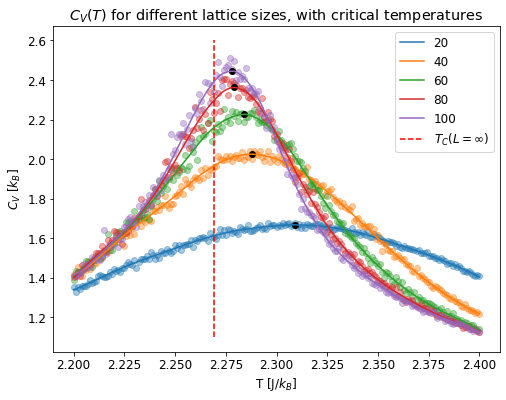
\includegraphics[width=80mm]{../../Code/Figures/Cv.png}
		\caption{The expected value of heat capacity per spin, for a $L \times L$ lattice. The values were calculated with 1000000 sweeps of the lattice with the Metropolis algorithm. The lines show a fit to the data using a Savgol filter. The black dots are the tops of the "spikes", which we take as the critical temperature for that lattice size. The red dotted line shows the critical temperature of an infinitely large lattice.}
		\label{fig:Cv}
	\end{figure}
	The expected value of magnetic susceptibility per spin for each temperature is shown in figure \ref{fig:E}.
	
	We performed the same analysis of the critical temperatures as for the heat capacity and found a critical temperature for an infinite lattice of $2.2669 J/k_B$, $0.0023 J/k_B$ away from the actual value of 2.2692.
	\begin{figure}[H]
		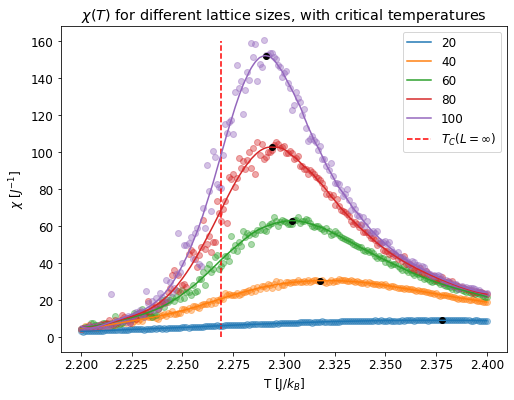
\includegraphics[width=80mm]{../../Code/Figures/X.png}
		\caption{The expected value of magnetic susceptibility per spin, for a $L \times L$ lattice. The values were calculated with 1000000 sweeps of the lattice with the Metropolis algorithm. The lines show a fit to the data using a Savgol filter. The black dots are the tops of the "spikes", which we take as the critical temperature for that lattice size. The red dotted line shows the critical temperature of an infinitely large lattice.}
		\label{fig:X}
	\end{figure}
	
	
\section{Discussion} %------------------Diskusjon-----------------------
\subsection{Testing and benchmarks}
	We tested our algorithm for the 2x2 lattice, which we solved analytically. We see in figure \ref{fig:2x2E}, \ref{fig:2x2M}, \ref{fig:2x2Cv} and \ref{fig:2x2X}, that our algorithm reproduced the analytical results very closely.
	
	We also timed our algorithm with and without parallellization. We found that parallizing the code gave a speedup of about 4.4, as shown in figure \ref{fig:time}. This was a practical necessity for producting the results in this report, as the longest calculation took 7 hours.

\subsection{Time to equilibrium}
	We plotted the energy and magnetic moment per spin for each sweep of the lattice in figures \ref{fig:EMC} and \ref{fig:MMC}. We see that for T=1 the system quickly settles in a state where all spins are pointing in the same direction, if it did not start in such a state. For T=2.4 however, both energy and magnetic moment fluctuates wildly, but in the same general area. The behavior does not seem to change after about 1000 cycles, but we chose to discard the first 10000 cycles in our calculations moving forward, since this simulation of the 20x20 lattice might not be representative of the time to equilibrium for larger lattices. 10000 cycles are also not very many compared to the 1000000 cycles we used for our main results, so we chose to be on the safe side.
	
	Figure \ref{fig:AMC} illustrates what we already saw in figures \ref{fig:EMC} and \ref{fig:MMC}. For T=1, the system accepts flips which take it closer to a state with all spins pointing in the same direction, and then accepts very few flips once it is in such a state, as shown by the line for T=1 starting in an unordered state. For T=2.4 however, the system never "settles" near a particular microstate, instead flipping between many nearly equally likely states.
	
	The plot of the number of occurences of each energy, figure \ref{fig:PE}, illustrates this behavior. For T=1, the probability distribution of the different energies is very narrow, with a standard deviation of 0.007J. The most likely states are very close together in energy. For T=2.4 however, there is a much wider spread of likely energies, shown by the wide histogram, and the standard deviation of 0.14J.

\subsection{The critical temperature}
	Figure \ref{fig:E} shows that the expected energy per spin increases with temperature, and that the increase is the fastest around the critical temperature of around 2.27-2.3. Is also shows that the energy per spin increases with lattice size. This backs up the claim that around the critical temperature, the spins become much less aligned.
	
	The magnetic moment in figure \ref{fig:M} also shows how the spins become less aligned around the critical temperature, and with an increase in lattice size. As discussed in the methods section, magnetic moment decreases very rapidly around the critical temperature. The critical temperature is hard to decide from the magnetic moment plot alone however.
	
	The acceptance rate of flips as a function of temperature is shown in figure \ref{fig:A}. This figure shows part of the transition from the low acceptance rate we saw for T=1 in figure \ref{fig:AMC}, to the high acceptance rate we saw for T=2.4. Again, we see how increased temperature leads to increased entropy, illustrated by flips being accepted and the system having no strong "preference" for which direction the spins should be aligned in.
	
	Figure \ref{fig:Cv} shows how the heat capacity per spin increases near the critical temperature. The larger the lattice, the larger the increase, and the lower the critical temperature, up to a point. We see that the critical temperatures are closer between large lattices than smaller lattices. This is what we would expect from equation \ref{eq:tc}.
	
	The fit of equation \ref{eq:tc} yielded a critical temperature for an infinite lattice of 2.2699, which differs only by 0.0007 from the analytical value of 2.2692. This result shows the strength of the Matropolis algorithm for simulating the Ising model. The result does however come with some uncertainty from the choice of Savgol filter, the resolution of our data, and of course the linear fit. So it would take calculations with larger lattices and more temperatures to definitively show that the analytical result is properly reproduced.
	
	An example of this uncertanty comes from our result from using the magnetic susceptibility as a way of finding the critical temperature of an infinite lattice. We made the same assumptions as for the heat capacity, but had an error which was more than three times as large. The results for the critical temperature is still very promising however, it shows that the theory and our simulations are well aligned.

\section{Conclusion} %------------------Konklusjon-----------------------
	We have studied the Ising model using the Metropolis algorithm. We confirmed that the algorithm reproduced analytical results for a 2x2 lattice, and parallellized the algorithm to achieve a speedup of around 4.4.
	
	We found that the first few thousand cycles of the algorithm could skew our results, and thus chose to ignore them in our calculations.
	
	Using the Metropolis algorithm, we were able to show how the entropy of the system increased with temperature, and that around some critical temperature the magnetization dropped rapidly. By calculating the expected heat capacity per spin with 1000000 sweeps of the lattice for lattice sizes ranging from $20 \times 20$ to $100 \times 100$, we were able to predict that the critical temperature for an infinite lattice is $T_C(L = \infty) = 2.2699 J/k_B$, a value only $0.0007J/k_B$ away from the analytical result of $T_C(L = \infty) \approx 2.2692 J/k_B$. A similar calculation using the magnetic susceptibility per spin resulted in only a slightly worse result of $2.2669 J/k_B$.
	
	The results illustrated the strength of the Metropolis algorithm, and the physical properties of the Ising model with changing temperatures. Future improvements to our calculations could include more cycles and temperatures, and a method of calculating the critical temperatures whose uncertainty can be calculated in a rigorous manner.

\begin{figure*} \bibliography{biblio} \end{figure*}
	
\end{document}